\nofiles\documentclass{article}
\usepackage{amsmath}
\usepackage{pgfplots}
\newcommand{\colorone}{blue}
\newcommand{\colortwo}{red}
\usetikzlibrary{decorations.pathreplacing}

\begin{document}

\section{Reflection Property of a Parabola}

Let $y=\frac{x^2}{4p}$ so that $y'=\frac x{2p}$.  We want to show that any ray parallel to the axis $y=0$ will reflect to the focus $(0,p)$.  Suppose that we have a ray intersecting the parabola at $(x,y)$.  Suppose that the line from the focus to this point of intersection makes an angle of $\theta$ with the horizontal, so that its slope is $\tan\theta=\frac{y-p}x$.  Let $\phi$ be the angle of the tangent line to the horizontal, so that its slope is $\tan\phi=\frac x{2p}$.

% focus at (0,1), intersection at (2sqrt2,2)
\begin{center}
\begin{tikzpicture}
\begin{axis}[width=.7\textwidth,tick label style={font=\scriptsize},
axis y line=middle,axis x line=middle,name=myplot,
ymin=-1.5,ymax=4.2,xmin=-1.2,xmax=4.2,axis equal]
\addplot [draw={\colorone},thick, smooth,domain=-1.2:4.2]{x*x/4};
\filldraw (axis cs:0,1) circle (1.5pt) node {};
\draw[draw={\colortwo},thick](axis cs:0,1)--(axis cs:2.828,2)--(axis cs:2.828,4.2);
\end{axis}
\node [right] at (myplot.right of origin) {\scriptsize $x$};
\node [above] at (myplot.above origin) {\scriptsize $y$};
\end{tikzpicture}
\end{center}

Zooming in to the point of reflection and using that the angles of a triangle add to $\pi$, we have the following:

\begin{center}
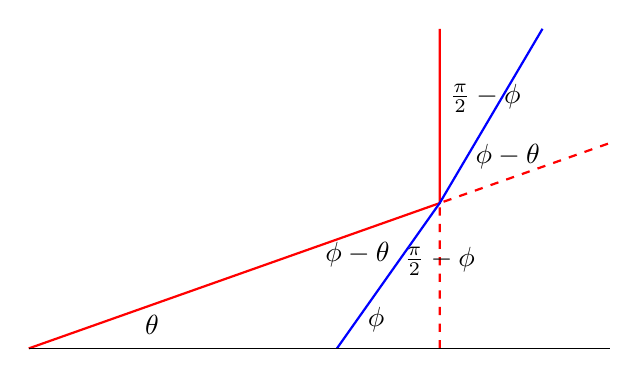
\begin{tikzpicture}
\begin{axis}[width=.8\textwidth,tick label style={font=\scriptsize},
axis y line=none,axis x line=none,name=myplot,
ymin=.9,ymax=3.2,xmin=-.2,xmax=4.2,axis equal]
\draw[draw={\colortwo},thick]
 (axis cs:0,1)--node[pos=.3,color={black},below]{$\theta$}node[pos=.8,color={black},below]{$\phi-\theta$}
 (axis cs:2.828,2)--node[pos=.6,color={black},right]{$\frac\pi2-\phi$}
 (axis cs:2.828,3.2);
\draw[draw={\colortwo},thick,dashed]
 (axis cs:2.828,1)--node[pos=.6,color={black}]{$\frac\pi2-\phi$}
 (axis cs:2.828,2)--node[pos=.4,color={black},above]{$\phi-\theta$}(axis cs:4,2.414);
% y-2 = sqrt2(x-2sqrt2)
% y=1 => x = 2sqrt2 - 1/sqrt2 = 2sqrt2 - sqrt2 /2 = sqrt2 * 3/2
% x=4 => y = 2+sqrt2(4-2sqrt2)
% y=3 => x = 2sqrt2 + 1/sqrt2 = 2sqrt2 + sqrt2 /2 = sqrt2 * 5/2
\draw[draw={\colorone},thick]
 (axis cs:2.121,1)--node[pos=.2,color={black},right]{$\phi$}
 (axis cs:2.828,2)--(axis cs:3.536,3.2);
\draw[draw={black}](axis cs:0,1)--(axis cs:4,1);
\end{axis}
\end{tikzpicture}
\end{center}

The reflection property will hold if $\phi-\theta=\frac\pi2-\phi$, or $2\phi=\theta+\frac\pi2$.  To show this is the case, we take the tangent of both sides.  On the left hand side, we have that
\[
 \tan2\phi=\frac{2\tan\phi}{1-\tan^2\phi}
 =\frac{\frac xp}{1-\frac{x^2}{4p^2}}=\frac{4px}{4p^2-x^2}.
\]
On the right side, we have that
\[
 \tan\left(\theta+\frac\pi2\right)=-\frac1{\tan\theta}=\frac x{y-p}
 =\frac x{\frac{x^2}{4p}-p}=\frac{4px}{4p^2-x^2},
\]
proving our claim.

\section{Reflection Property of Ellipses}

Let $\frac{x^2}{a^2}+\frac{y^2}{b^2}=1$, so that $y'=-\frac{xb^2}{ya^2}$.  We want to show that any ray leaving one focus will reflect to the other focus.  Suppose that $a>b$, and let $c^2=a^2-b^2$, so that the focuses are at $(\pm c,0)$.  Suppose that we have a ray intersecting the ellipse at $(x,y)$.  Let the tangent line have an angle of $\phi$ from the horizontal, so that its slope is $\tan\phi=-\frac{xb^2}{ya^2}$.  Let the ray from the focus $(-c,0)$ make an angle of $\theta_1$ with the horizontal, so that its slope is $\tan\theta_1=\frac y{x+c}$.  Finally, let the ray from the focus $(c,0)$ make an angle of $\theta_2$ with the horizontal, so that its slope is $\tan\theta_2=\frac y{x-c}$.

% x^2/4 + y^2 = 1
% a=2, b=1
% at (1,sqrt3/2)
\begin{center}
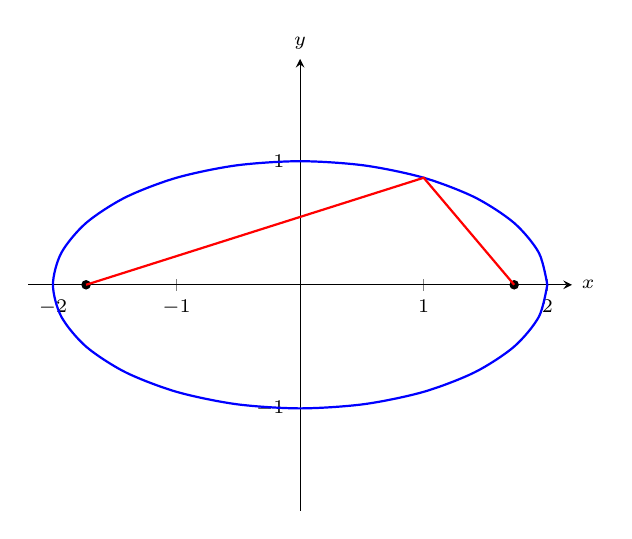
\begin{tikzpicture}
\begin{axis}[width=.7\textwidth,tick label style={font=\scriptsize},
axis y line=middle,axis x line=middle,name=myplot,
ymin=-1.5,ymax=1.5,xmin=-2.2,xmax=2.2,axis equal]
\addplot [draw={\colorone},thick, smooth,domain=0:360]({2*cos(x)},{sin(x)});
\filldraw (axis cs:1.732,0) circle (1.5pt) node {};
\filldraw (axis cs:-1.732,0) circle (1.5pt) node {};
\draw[draw={\colortwo},thick](axis cs:-1.732,0)--(axis cs:1,0.866)--(axis cs:1.732,0);
\end{axis}
\node [right] at (myplot.right of origin) {\scriptsize $x$};
\node [above] at (myplot.above origin) {\scriptsize $y$};
\end{tikzpicture}
\end{center}

Zooming in to the point of reflection and using that the angles of a triangle or a straight line add to $\pi$, we have the following:

\begin{center}
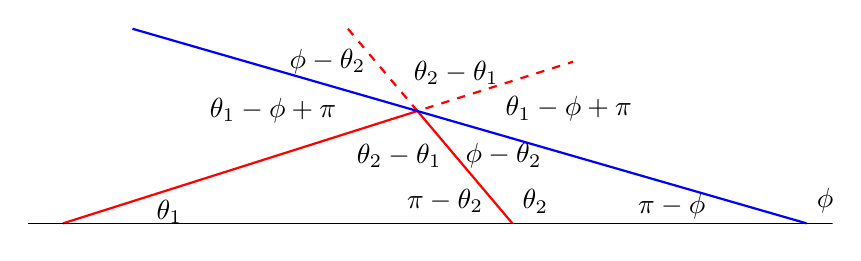
\begin{tikzpicture}
\begin{axis}[width=\textwidth,tick label style={font=\scriptsize},
axis y line=none,axis x line=none,name=myplot,
ymin=-.5,ymax=1.5,xmin=-2.2,xmax=4.2,axis equal]
\draw[draw={\colortwo},thick]
 (axis cs:-1.732,0)--
 node[pos=.3,color={black},below]{$\theta_1$}
 node[pos=.8,color={black},below right]{$\theta_2-\theta_1$}
 node[pos=.8,color={black},above left]{$\theta_1-\phi+\pi$}
 (axis cs:1,0.866)--
 node[pos=.4,color={black},right]{$\phi-\theta_2$}
 node[pos=.8,color={black},left]{$\pi-\theta_2$}
 node[at end,color={black},above right]{$\theta_2$}
 (axis cs:1.732,0);
\draw[draw={\colortwo},thick,dashed]
 (axis cs:0.464102,1.5)--
 node[pos=.4,color={black},left]{$\phi-\theta_2$}
 node[pos=.8,color={black},above right]{$\theta_2-\theta_1$}
 (axis cs:1,0.866)--
 node[pos=.5,color={black},below right]{$\theta_1-\phi+\pi$}
 (axis cs:2.2,1.246);
% y-sqrt3/2 = -(x-1)/2sqrt3
\draw[draw={\colorone},thick](axis cs:-1.1962,1.5)--
 node[at end,color={black},above right]{$\phi$}
 node[pos=.8,color={black},below]{$\pi-\phi$}(axis cs:4,0);
\draw[draw={black}](axis cs:-2,0)--(axis cs:4.2,0);
\end{axis}
\end{tikzpicture}
\end{center}

The reflection property will hold if $\theta_1-\phi+\pi=\phi-\theta_2$, or $\theta_1+\theta_2+\pi=2\phi$.  To show this is the case, we take the tangent of both sides.  On the left hand side, we have
\[
 \tan(\theta_1+\theta_2+\pi)=\tan(\theta_1+\theta_2)
 =\frac{\tan\theta_1+\tan\theta_2}{1-\tan\theta_1\tan\theta_2}
 =\frac{\frac y{x+c}+\frac y{x-c}}{1-\frac y{x+c}\frac y{x-c}}
% =\frac{y(x-c)+y(x+c)}{(x+c)(x-c)-y^2}
 =\frac{2xy}{x^2-y^2-c^2}.
\]
On the right hand side, we have
\[
 \tan2\phi=\frac{2\tan\phi}{1-\tan^2\phi}
 =\frac{-\frac{2xb^2}{ya^2}}{1-\frac{x^2b^4}{y^2a^4}}
% =\frac{-2xb^2ya^2}{y^2a^4-x^2b^4}
 =\frac{-2xy}{\frac{y^2a^2}{b^2}-\frac{x^2b^2}{a^2}}
 =\frac{-2xy}{(1-\frac{x^2}{a^2})a^2-(1-\frac{y^2}{b^2})b^2}
% =\frac{-2xy}{a^2-x^2-b^2+y^2}
 =\frac{2xy}{x^2-y^2-(a^2-b^2)},
\]
proving our claim.

\section{Reflection Property of Hyperbolas}

Let $\frac{x^2}{a^2}-\frac{y^2}{b^2}=1$, so that $y'=\frac{xb^2}{ya^2}$.  We want to show that any ray aiming at one focus will reflect toward the other focus.  Let $c^2=a^2-b^2$, so that the focuses are at $(\pm c,0)$.  Suppose that we have a ray intersecting the hyperbola at $(x,y)$.  Let the tangent line have an angle of $\phi$ from the horizontal, so that its slope is $\tan\phi=\frac{xb^2}{ya^2}$.  Let the ray toward the focus $(-c,0)$ make an angle of $\theta_1$ with the horizontal, so that its slope is $\tan\theta_1=\frac y{x+c}$.  Finally, let the ray toward the focus $(c,0)$ make an angle of $\theta_2$ with the horizontal, so that its slope is $\tan\theta_2=\frac y{x-c}$.

% x^2 - y^2 = 1
% a=1, b=1
% at (sqrt2,1)
\begin{center}
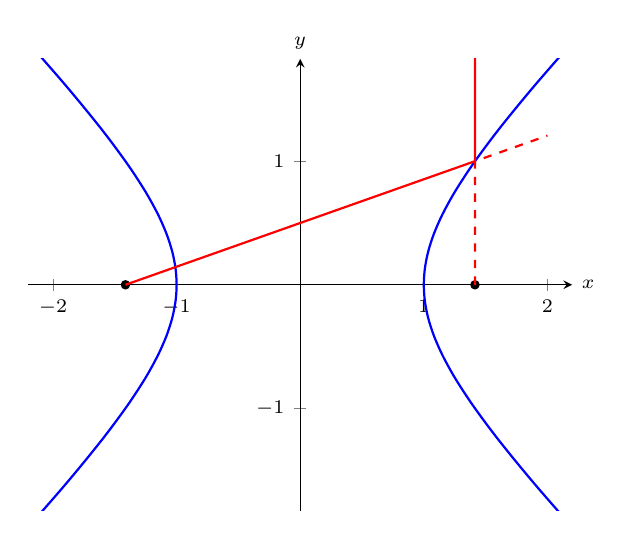
\begin{tikzpicture}
\begin{axis}[width=.7\textwidth,tick label style={font=\scriptsize},
axis y line=middle,axis x line=middle,name=myplot,
ymin=-1.5,ymax=1.5,xmin=-2.2,xmax=2.2,axis equal]
\addplot [draw={\colorone},thick, smooth,domain=-89:89]({sec(x)},{tan(x)});
\addplot [draw={\colorone},thick, smooth,domain=91:269]({sec(x)},{tan(x)});
\filldraw (axis cs:1.414,0) circle (1.5pt) node {};
\filldraw (axis cs:-1.414,0) circle (1.5pt) node {};
\draw[draw={\colortwo},thick](axis cs:-1.414,0)--(axis cs:1.414,1)--(axis cs:1.414,2.2);
\draw[draw={\colortwo},thick,dashed](axis cs:1.414,0)--(axis cs:1.414,1)--(axis cs:2,1.207);
\end{axis}
\node [right] at (myplot.right of origin) {\scriptsize $x$};
\node [above] at (myplot.above origin) {\scriptsize $y$};
\end{tikzpicture}
\end{center}

Zooming in to the point of reflection and using that the angles of a triangle or a straight line add to $\pi$, we have the following:

\begin{center}
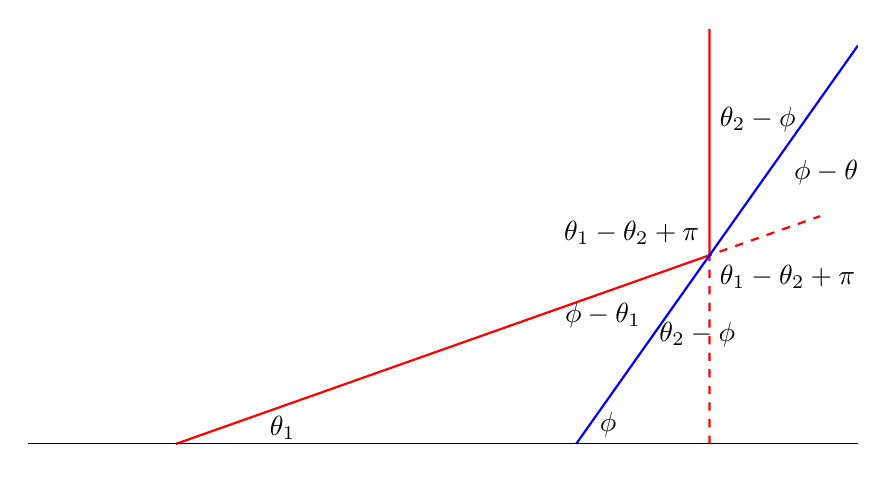
\begin{tikzpicture}
\begin{axis}[width=\textwidth,tick label style={font=\scriptsize},
axis y line=none,axis x line=none,name=myplot,
ymin=-.5,ymax=1.5,xmin=-2.2,xmax=2.2,axis equal]
\draw[draw={\colortwo},thick](axis cs:-1.414,0)--
 node[pos=.2,below,color={black}]{$\theta_1$}
 node[pos=.8,below,color={black}]{$\phi-\theta_1$}
 node[pos=1,above left,color={black}]{$\theta_1-\theta_2+\pi$}(axis cs:1.414,1)--
 node[pos=.6,right,color={black}]{$\theta_2-\phi$}
 (axis cs:1.414,2.2);
\draw[draw={\colortwo},thick,dashed](axis cs:1.414,0)--
 node[pos=1,below right,color={black}]{$\theta_1-\theta_2+\pi$}(axis cs:1.414,1)--
 (axis cs:2,1.207);
% y-1 = sqrt2(x-sqrt2)
\draw[draw={\colorone},thick](axis cs:.707,0)--
 node[pos=.1,right,color={black}]{$\phi$}
 node[pos=.7,below,color={black},xshift=1em]{$\theta_2-\phi$}(axis cs:1.414,1)--
 node[pos=.5,below right,color={black}]{$\phi-\theta_1$}(axis cs:2.2,2.111);
\draw[draw={black}](axis cs:-2.2,0)--(axis cs:2.2,0);
\end{axis}
\end{tikzpicture}
\end{center}

The reflection property will hold if $\phi-\theta_1=\theta_2-\phi$, or $\theta_1+\theta_2=2\phi$. To show this is the case, we take the tangent of both sides.  On the left hand side, we have
\[
 \tan(\theta_1+\theta_2)
 =\frac{\tan\theta_1+\tan\theta_2}{1-\tan\theta_1\tan\theta_2}
 =\frac{\frac y{x+c}+\frac y{x-c}}{1-\frac y{x+c}\frac y{x-c}}
% =\frac{y(x-c)+y(x+c)}{(x+c)(x-c)-y^2}
 =\frac{2xy}{x^2-y^2-c^2}.
\]
On the right hand side, we have
\[
 \tan2\phi=\frac{2\tan\phi}{1-\tan^2\phi}
 =\frac{\frac{2xb^2}{ya^2}}{1-\frac{x^2b^4}{y^2a^4}}
% =\frac{2xb^2ya^2}{y^2a^4-x^2b^4}
 =\frac{2xy}{\frac{y^2a^2}{b^2}-\frac{x^2b^2}{a^2}}
 =\frac{2xy}{(\frac{x^2}{a^2}-1)a^2-(\frac{y^2}{b^2}+1)b^2}
% =\frac{2xy}{a^2-x^2-b^2+y^2}
 =\frac{2xy}{x^2-y^2-(a^2+b^2)},
\]
proving our claim.

\section{The Parabola as a Limit of an Ellipse}

Suppose that we fix a distance $p$ between one focus of an ellipse and the near end of the major axis.  We want to show that as the distance to the other focus increases without bound, the ellipse becomes a parabola.  We'll start with the ellipse $\frac{x^2}{a^2}+\frac{y^2}{b^2}=1$, with $a>b$ and $c^2=a^2-b^2$.  Let $p=a-c$ be the distance from the focus to the near end of the major axis.  Shifting so that this near end lies on the origin and the near focus lies at $(p,0)$, the equation of the ellipse is $(\frac{x-a}a)^2+(\frac yb)^2=1$, or $y^2=b^2[1-(\frac{x-a}a)^2]$.
% (x-a)^2/a^2 + y^2/b^2 = 1
% a=5, b=3, c=4
\begin{center}
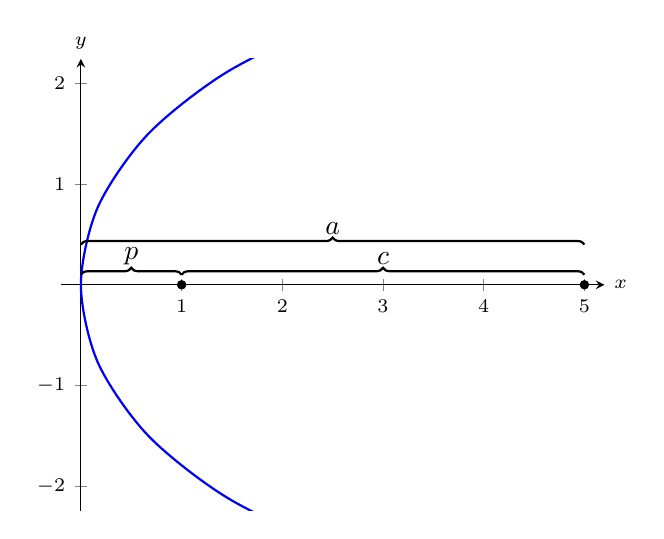
\begin{tikzpicture}
\begin{axis}[width=.7\textwidth,tick label style={font=\scriptsize},
axis y line=middle,axis x line=middle,name=myplot,
ymin=-2.2,ymax=2.2,xmin=-.2,xmax=5.2,axis equal]
\addplot [draw={\colorone},thick, smooth,domain=0:360]({5*cos(x)+5},{3*sin(x)});
%\filldraw (axis cs:3.732,0) circle (1.5pt) node {};
\filldraw (axis cs:1,0) circle (1.5pt) node {};
\filldraw (axis cs:5,0) circle (1.5pt) node {};
\draw[decoration=brace,decorate,thick](axis cs:0,.1)--node[above]{$p$}(axis cs:1,.1);
\draw[decoration=brace,decorate,thick](axis cs:1,.1)--node[above]{$c$}(axis cs:5,.1);
\draw[decoration=brace,decorate,thick](axis cs:0,.4)--node[above]{$a$}(axis cs:5,.4);
\end{axis}
\node [right] at (myplot.right of origin) {\scriptsize $x$};
\node [above] at (myplot.above origin) {\scriptsize $y$};
\end{tikzpicture}
\end{center}
We see that $b^2=a^2-c^2=(a-c)(a+c)=p(p+2c)$, so that
\[
 y^2=p(p+2c)\left[1-\left(\frac{x-p-c}{p+c}\right)^2\right]
% =p(p+2c)\left[1-\frac{x-p-c}{p+c}\right]\left[1+\frac{x-p-c}{p+c}\right]
% =p(p+2c)\left[\frac{p+c-x+p+c}{p+c}\right]\left[\frac{p+c+x-p-c}{p+c}\right]
% =p(p+2c)\left[\frac{2p+2c-x}{p+c}\right]\left[\frac x{p+c}\right]
 =\frac{(2p+2c-x)(p+2c)}{(p+c)^2}px
 \mathrel{\overset{c\to\infty}{\longrightarrow}}4px.
\]
Therefore, the ellipse becomes the expressions $x=\frac{y^2}{4p}$, the equation of a parabola with a vertex at the origin and focus at $(p,0)$.

\section{The Parabola as a Limit of a Hyperbola}

Suppose that we fix a distance $p$ between one focus of a hyperbola and the near vertex.  We want to show that as the distance to the other focus increases without bound, the branch of the hyperbola with this vertex becomes a parabola.  We'll start with the hyperbola $\frac{x^2}{a^2}-\frac{y^2}{b^2}=1$ and $c^2=a^2+b^2$.  Let $p=c-a$ be the distance from the focus to the vertex.  Shifting so that this vertex lies on the origin and the focus lies at $(p,0)$, the equation of the hyperbola is $(\frac{x+a}a)^2-(\frac yb)^2=1$, or $y^2=b^2[(\frac{x+a}a)^2-1]$.
% (x+a)^2/a^2 - y^2/b^2 = 1
% a=4, b=3, c=5
\begin{center}
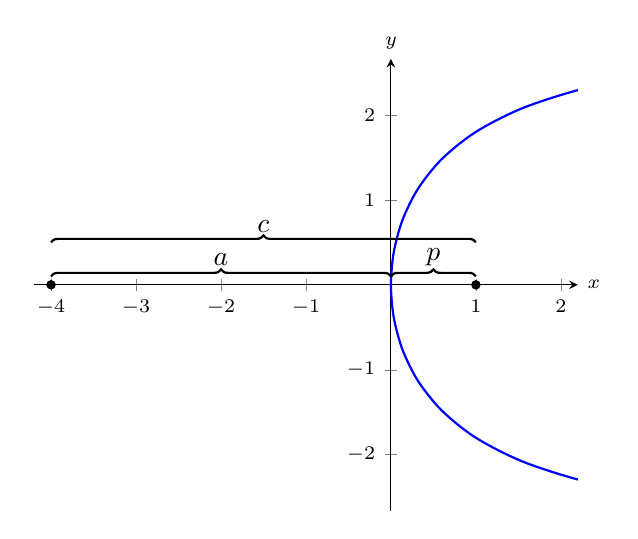
\begin{tikzpicture}
\begin{axis}[width=.7\textwidth,tick label style={font=\scriptsize},
axis y line=middle,axis x line=middle,name=myplot,
ymin=-2.2,ymax=2.2,xmin=-4.2,xmax=2.2,axis equal]
\addplot [draw={\colorone},thick, smooth,domain=-89:89]({4*sec(x)-4},{3*sin(x)});
%\filldraw (axis cs:3.732,0) circle (1.5pt) node {};
\filldraw (axis cs:-4,0) circle (1.5pt) node {};
\filldraw (axis cs:1,0) circle (1.5pt) node {};
\draw[decoration=brace,decorate,thick](axis cs:0,.1)--node[above]{$p$}(axis cs:1,.1);
\draw[decoration=brace,decorate,thick](axis cs:-4,.5)--node[above]{$c$}(axis cs:1,.5);
\draw[decoration=brace,decorate,thick](axis cs:-4,.1)--node[above]{$a$}(axis cs:0,.1);
\end{axis}
\node [right] at (myplot.right of origin) {\scriptsize $x$};
\node [above] at (myplot.above origin) {\scriptsize $y$};
\end{tikzpicture}
\end{center}
% a = c-p
We see that $b^2=c^2-a^2=(c-a)(c+a)=p(2c-p)$, so that
\[
 y^2=p(2c-p)\left[\left(\frac{x+c-p}{c-p}\right)^2-1\right]
% =p(2c-p)\left[\frac{x+c-p}{c-p}-1\right]\left[\frac{x+c-p}{c-p}+1\right]
% =p(2c-p)\left[\frac{x+c-p-c+p}{c-p}\right]\left[\frac{x+c-p+c-p}{c-p}\right]
% =p(2c-p)\left[\frac x{c-p}\right]\left[\frac{x+2c-2p}{c-p}\right]
 =\frac{(x+2c-2p)(2c-p)}{(c-p)^2}px
 \mathrel{\overset{c\to\infty}{\longrightarrow}}4px.
\]
Therefore, the hyperbola becomes the expressions $x=\frac{y^2}{4p}$, the equation of a parabola with a vertex at the origin and focus at $(p,0)$.

\section{Polar Equations of Conic Sections}

\end{document}
